\documentclass[letterpaper,journal]{IEEEtran}
\usepackage{graphicx,booktabs,amsmath,amssymb,url,multirow,array,etoolbox,microtype}
\patchcmd{\thebibliography}{\footnotesize}{\scriptsize}{}{}
\renewcommand{\arraystretch}{0.9}
\usepackage[hidelinks]{hyperref}
\setlength{\textfloatsep}{8pt plus 1pt minus 2pt}
\setlength{\dbltextfloatsep}{8pt plus 1pt minus 2pt}
\setlength{\floatsep}{8pt plus 1pt minus 2pt}
\setlength{\intextsep}{8pt plus 1pt minus 2pt}
\setlength{\abovecaptionskip}{4pt}
\newcommand{\cb}{\texttt{cost\_bid}}
\newcommand{\gb}{\texttt{group\_bid}}
\begin{document}
\title{Who Backs Into the Bay? Benchmarking Negotiation Policies for Head-On Robot Encounters in Single-Lane Corridors}
\author{Roshan George, Martin Glavin, Edward Jones, and Brian Deegan%
\thanks{All authors are with the Connaught Automotive Research (CAR) group and the Ryan Institute, University of Galway, Ireland (e-mail: brian.deegan@universityofgalway.ie).}%
\thanks{DRAFT, not for distribution.}}
\maketitle

\begin{abstract}
When two mobile robots meet head-on in a corridor that admits only one, one of them must reverse into a pull-in bay or out of the corridor. We benchmark who should yield, and into which refuge, by running the same agent code in a 2D simulator and in ROS~2/Gazebo with TurtleBot3 Waffles. We compare a non-communicating reactive baseline, fixed priority, a rulebook, corridor reservation, cost bidding, a convoy group bid, a Clarke-pivot mechanism, and a learned negotiator against the best forced yielder, a hindsight reference that tries both yield decisions. In the single-bay study (420 episodes per policy), the reactive baseline succeeds in 93.8\% of episodes with at least 3.6$\times$ the reference's delay, and every negotiating policy succeeds in all episodes. When bids use the simulator's own cost model, cost bidding picks the reference's yielder in every single- and two-bay episode, and with asymmetric robots its urgency-weighted excess delay is 0.04\,s against 27.1\,s for fixed priority. With log-normal bid noise of $\sigma=0.5$ it is no better than a noise-free closest-refuge rule. Clarke payments remove the gain from scaled misreports under the same model but leave a budget surplus. Under 90--99\% packet loss no safeguard-ablation arm collided. In 460 Gazebo runs on a reduced grid, no non-reactive run failed, and 393 of 406 negotiating runs chose the same first yielder as in 2D; T-junction delays did not transfer; code, scripts, and results are released.
\end{abstract}

\begin{IEEEkeywords}
Multi-robot systems, negotiation, deadlock, path planning for multiple mobile robots, benchmarking.
\end{IEEEkeywords}

\section{Introduction}
\IEEEPARstart{N}{arrow} aisles, doorways, and service corridors force autonomous mobile robots (AMRs) into conflicts that local collision avoidance cannot resolve: if two robots meet head-on where only one fits, someone must back off. Reciprocal collision avoidance and control-barrier-function controllers deadlock in such symmetric configurations~\cite{grover2023before,dergachev2021distributed,chandra2025deadlock}, while centralized planners and traffic managers avoid the conflict at the price of a global plan~\cite{cap2016provably,okumura2022pibt,phillips2011sipp,hiertraffic2023,rmftraffic,openrmf}. Between these extremes lies decentralized negotiation: the robots exchange messages and agree who yields. Rules of the road~\cite{kato1992coordinating,shoham1995social}, auctions~\cite{gerkey2002sold,gautier2022negotiated}, learned policies~\cite{vmasgiveway,bettini2023heterogeneous}, language-model negotiation~\cite{marlin2024,gamechat2025}, and foundation-model high-level planners for deadlock resolution~\cite{garg2024llm} have all been proposed, but each paper builds its own scene and metrics, and to our knowledge no study compares the families under the same physics and communication model~\cite{chandra2026social}. We take the deadlock of reciprocal avoidance in this configuration from the cited work; our benchmark does not include an ORCA, RVO, or CBF controller, so it does not reproduce that deadlock.

This letter contributes:
\begin{enumerate}
\item an open benchmark of the head-on corridor encounter with pull-in bays, in which the same agent state machine runs in a 2D simulator for Monte Carlo sweeps and in ROS~2 Jazzy/Gazebo Harmonic with TurtleBot3 Waffles\footnote{Code, scenarios, study scripts, and results: \url{[ANONYMIZED-URL]}.}; % TODO: insert repository URL / archival DOI before submission
\item a comparison of reactive, fixed-priority, rule-based, reservation, cost-bidding, group-bidding, Clarke-pivot, and learned negotiators over bay geometry, robot asymmetry, bid noise, strategic misreporting, repeated encounters, and packet loss and latency, with the full study design in Table~\ref{tab:design};
\item a factorial ablation of the protocol safeguards under extreme packet loss, and extensions to convoys, a T-junction, inconsistent maps, physically blocked bays, and exploring robots that share their map only after detecting each other;
\item a Gazebo check of where the 2D conclusions transfer: 460 runs, paired by seed with 2D, over a reduced grid of every study; yield decisions and excess delays transfer for the corridor studies whose random draws the two simulators share, and they differ where bid noise, heavy packet loss, or lidar detection timing is realized differently in each simulator; T-junction delays do not transfer.
\end{enumerate}

\section{Related Work}
\emph{Deadlock in narrow passages.} Symmetric encounters are a known failure mode of decentralized avoidance. Grover et al.~\cite{grover2023before} characterize CBF deadlocks; Dergachev and Yakovlev~\cite{dergachev2021distributed} switch to local multi-agent path finding (MAPF) when ORCA stalls; Chandra et al.~\cite{chandra2025deadlock} perturb controls onto liveness sets in doorways and hallways. These works resolve who goes first by slowing down, not by choosing which robot reverses into which refuge.
\emph{Centralized coordination.} MAPF and AGV traffic management treat bays as graph nodes~\cite{stern2019mapf,okumura2022pibt,experience2024narrow,macga2025}; zone control grants exclusive access to corridor segments~\cite{fanti2002event,geozone2023}, which our reservation baseline mimics; safe-interval planning reserves corridor segments in time~\cite{phillips2011sipp}, fleet managers such as Open-RMF negotiate conflicting schedules centrally~\cite{openrmf,rmftraffic}, and precedence-preserving coordinators provide safety under delays~\cite{cap2016provably,mannucci2019provably}. They require a global planner or schedule database and typically charge reversing as ordinary motion.
\emph{Negotiation and mechanisms.} Social laws~\cite{shoham1995social}, market-based allocation~\cite{gerkey2002sold}, and negotiated path planning~\cite{gautier2022negotiated} assume truthful costs. Vickrey--Clarke--Groves mechanisms~\cite{vickrey1961counterspeculation,clarke1971multipart,groves1973incentives,nisan2001algorithmic} make truthful reporting dominant, but no efficient, truthful mechanism is budget balanced in general~\cite{green1977characterization,myerson1983efficient}. Karma schemes trade non-monetary credit across repeated encounters to make right-of-way allocation fair~\cite{censi2019karma,elokda2024karma}; cooperative give-way at road bottlenecks has also been studied for connected vehicles~\cite{bottleneckiv2023}.
\emph{Learning and LLMs.} MARL give-way tasks exist in VMAS~\cite{vmasgiveway}; MARLIN uses LLM negotiation to guide MARL training in narrow-corridor swaps, with physical TurtleBot3 experiments~\cite{marlin2024}; GameChat sets priority through LLM dialogue in doorways~\cite{gamechat2025}. None compares against rule-based, bidding, and hindsight baselines under communication impairment, which is the gap we address.

\section{Benchmark}
\subsection{Scenarios}
The base scenario (Fig.~\ref{fig:scen}a) is an 8\,m$\times$0.65\,m corridor between two 2.5\,m rooms. A TurtleBot3 Waffle (0.281\,m$\times$0.306\,m body, 0.25\,m swept radius when turning in place, 0.26\,m/s forward, 0.15\,m/s reverse) fits; two cannot pass, because two bodies side by side leave 0.04\,m of the 0.65\,m width, less than the 0.05\,m wall clearance each robot keeps, and the controller tracks the centerline with no passing maneuver. Bays are 0.8\,m wide and 0.6\,m deep, with configurable position, side, and number; the end rooms also serve as refuges. Robot A starts 1\,m before the corridor at $t=0$, and B starts 1\,m beyond the far end after a delay drawn from $U[0,8]$\,s. A needs about 35\,s to clear the corridor and B enters it within about 12\,s, so every draw produces a head-on encounter. Variants add a second bay (Fig.~\ref{fig:scen}b), a two-robot convoy against one oncoming robot (Fig.~\ref{fig:scen}c), and a T-junction (Fig.~\ref{fig:scen}d) whose side branch is approximated as a 2\,m-deep bay that a robot may leave or have as its destination; it is not a full 2D junction. Robots can differ in urgency, payload, and speed limits. Communication is a broadcast bus with a fixed latency plus a uniform jitter $U[0,j]$ and independent per-receiver loss; the default is 0.05\,s latency, $j=0.02$\,s, and no loss.

\begin{figure}[t]\centering
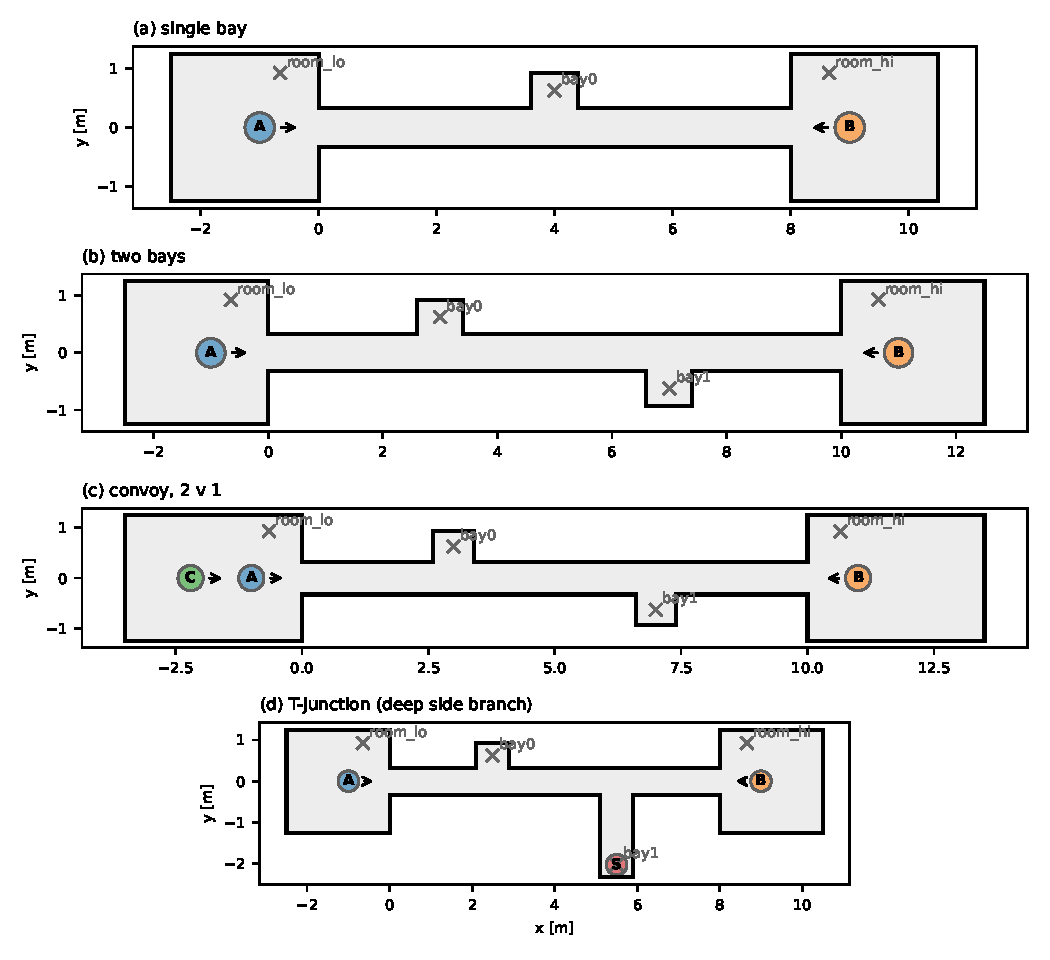
\includegraphics[width=0.95\columnwidth]{fig/scenarios.pdf}
\caption{Benchmark scenarios (gray: free space; $\times$: refuge parking poses). Arrows show travel direction. (d) shows the turn-in variant, in which robot S starts in the side branch and A's destination is the branch; in the exit variant only S uses the branch.}
\label{fig:scen}
\end{figure}

\subsection{Agent and protocol}\label{sec:proto}
Each robot runs the same state machine (cruise, negotiate, yield, proceed, done) at 20\,Hz, with lidar perception (3.5\,m range) and a unicycle model. The 2D simulator integrates the unicycle with forward Euler at the same 0.05\,s step, under limits of 0.5\,m/s$^2$ linear and 3\,rad/s$^2$ angular acceleration and 1.82\,rad/s turn rate; its lidar sees peers within range as 0.25\,m circles, without occlusion. Robots broadcast STATE messages at 5\,Hz. Negotiating robots detect a conflict from the peer positions in these STATE messages, not from the lidar: a conflict exists when an oncoming peer is within the detection range along the corridor (6\,m by default, beyond the 3.5\,m lidar range). The lidar serves the reactive baseline, the bay check, and explore mode. On conflict, the robots exchange BID messages containing a snapshot of their pose, speed, urgency, payload, and known refuges. Both robots then run the same deterministic decision function on the same pair of snapshots, so they agree without a third message when no message is lost. A yield plan names the yielder and its refuge; feasibility checks that the refuge lies behind the yielder and is not taken.

With message loss the robots may decide on different snapshots. Three safeguards address this, and each can be switched off for ablation. \emph{Commit}: each robot broadcasts its decision and acts only once it holds the peer's, the lower-ID robot's decision wins a disagreement, and an unconfirmed decision expires after 3\,s. \emph{State guard}: a yielder whose peer's STATE shows it yielding into the same refuge, or yielding to it, gives way and proceeds instead. \emph{Bay check}: a bay that the lidar shows occupied counts as taken, and a yielder that finds a robot in its bay proceeds. A robot waiting to pass also renegotiates if its supposed yielder approaches it. The timers are the same in every study. A negotiating robot resends its BID every 0.3\,s until the peer acknowledges its decision. A STATE counts as fresh for 1\,s after its receipt, and the state guard, the renegotiation check, and the release of a waiting robot use only fresh STATE. A waiting robot passes once a fresh STATE or its lidar shows the yielder off the lane. A parked yielder leaves once the peer's STATE shows it past the refuge; without a fresh STATE it leaves when its lidar shows the peer past, or after a delay drawn per yield from $U[6,12]$\,s, provided the lidar shows the lane clear. If no peer BID arrives within 3\,s, or a waiting robot's yielder has not left the lane within 60\,s, the robot falls back to the reactive behavior and negotiates again only when a peer's BID reaches it; if no feasible refuge remains, it acts reactively and does not renegotiate with that peer for 10\,s. We give no formal safety or liveness proof for this protocol; its behavior is characterized empirically in Sec.~\ref{sec:comms}.

\subsection{Policies}\label{sec:pol}
\emph{Reactive}: no messages; a blocked robot waits a patience time drawn from $U[2,6]$\,s and then backs to the nearest refuge behind it. \emph{Fixed priority}: the higher-ID robot always yields. \emph{Rulebook}: an ordered list of rules (no feasible refuge; urgency; payload; first in corridor; refuge within 2\,m behind; ID tie-break), the first discriminating rule decides; a variant puts ``closest refuge yields'' first. \emph{Reservation}: first come, first served, where the robot that entered the corridor first holds it; a robot still outside the corridor while an oncoming robot is inside waits in its end room; when neither is inside, both may enter, and robots that are both inside fall back to the rulebook. \emph{\cb}: for each candidate yielder $Y$ with proceeder $P$, both robots predict the delays $d_Y,d_P$ of $Y$'s best feasible plan with a constant-speed timeline model that uses the true speed limits, positions, and refuge geometry but ignores acceleration and turning transients, and evaluate $u_Y d_Y+u_P d_P$, where $u$ is urgency; the cheaper outcome is chosen. \emph{\gb}: as \cb, but a side's cost includes each yielding member's own urgency-weighted delay, the wait of the yielding side while the other side passes, and the delay of the proceeding side's followers. \emph{Clarke}: each robot reports its predicted urgency-weighted delay $r_i(o)$ under both outcomes $o$; the mechanism chooses $o^\ast=\arg\min_o\sum_i r_i(o)$ and charges robot $i$ the Clarke pivot $p_i=\sum_{j\neq i} r_j(o^\ast)-\min_o\sum_{j\neq i} r_j(o)$ in delay credit~\cite{clarke1971multipart}. Utility is quasi-linear: a robot's utility is minus the sum of its urgency-weighted delay and its payment, so 1\,s of credit is worth 1\,s of weighted delay. Credit is settled per encounter and is not carried into later encounters. For comparison we also test a \emph{naive transfer}, in which the proceeder pays the yielder's reported bid. \emph{Learned}: a tabular contextual bandit over a coarse observation (each robot's binned distance to its nearest feasible refuge behind it, which robot is more urgent, and both payload flags), trained on 800 encounters by running both forced outcomes; unseen observations fall back to fixed priority. It is a lightweight learned baseline, not deep multi-agent RL.

\subsection{Metrics and statistics}
We report success (all robots reach their goals within the 180\,s time limit, used in every study, without collision), deadlock (time limit reached), collision (overlap of the Waffle body rectangles; the 0.25\,m swept radius is used only for planning clearances and the simulated lidar, and in the blocked-bay study a robot within 0.5\,m of the obstacle's center also counts as colliding; the released minimum-clearance column is the axle-to-axle distance minus twice the swept radius, so robots stopped face to face can show negative values without contact, because the body extends only 0.08\,m ahead of the axle), total delay relative to free-flow travel time, urgency-weighted delay, reverse distance, and Jain's fairness index~\cite{jain1984fairness}. We apply Jain's index to the two robots' cumulative delays, clamped at zero; it then measures how evenly the cost is shared and equals 1 when both robots bear the same delay.

\emph{Excess delay.} The delay of an episode is $D=\sum_i w_i\,(T_i-T_i^{\mathrm{free}})$, where $T_i$ is robot $i$'s travel time, $T_i^{\mathrm{free}}$ its travel time with the corridor to itself, and $w_i=1$ (total delay) or $w_i$ equal to the robot's urgency (weighted delay). For every two-robot encounter $k$ we also run the two forced outcomes, A yields and B yields, each into that robot's best feasible refuge; the better of the two is the \emph{best forced yielder}. The excess delay of policy $\pi$ over $N$ encounters is
\begin{equation}
\Delta_\pi=\frac{1}{N}\sum_{k=1}^{N}\Bigl(D_\pi^{(k)}-\min\bigl(D_{A}^{(k)},D_{B}^{(k)}\bigr)\Bigr),
\label{eq:excess}
\end{equation}
paired by encounter, with the same weights $w_i$ in all three terms. $\Delta_\pi=0$ means the policy always made the better of the two yield decisions. The reference chooses only who yields, so $\Delta_\pi$ measures the quality of that decision, not the distance to a globally optimal joint motion plan, and a policy that also chooses \emph{when} to move could in principle have $\Delta_\pi<0$. It is the ex-post regret of decision theory; we avoid that term because it has different meanings in online learning and in mechanism design. Excess delay is defined for two-robot encounters; for the convoy we add a side-level reference, the better of ``the convoy yields'' and ``the lone robot yields''.

\emph{Code versions.} Apart from the pre-fix failures listed at the end of this paragraph, all reported numbers come from the final agent code. The last two commits, which added explore mode and Gazebo blocked-bay obstacles with per-run policy files, change nothing else on the default path, so the 2D studies other than explore mode ran on the pre-explore code. The hold-mode runs (Sec.~\ref{sec:explore}) ran on a branch of this code that adds the opt-in hold mode (merged before release). % VERIFIED 2026-10-23: released 2D studies ran at 338bcc2/07fd93f (ancestors of bf24bf4 on devin/1792011536-unified); then e400e99 (explore mode, default off) and 2ba4c6d (Gazebo), neither altering the default path; hold branch f5249a6 is merged on main
Where we report a failure that motivated a protocol change (collisions under extreme loss, convoy and T-junction deadlocks, blocked-bay deadlocks), that failure was observed on the code before the change; it motivates the fix and is not a result of the final code.

\emph{Statistics.} Table~\ref{tab:design} lists every study. Per-episode results are released with the scripts that produce the tables, except for the convoy and T-junction studies and the bid-capture reruns of Secs.~\ref{sec:two} and~\ref{sec:three}, whose scripts regenerate them from fixed seeds. % TODO(artifact): release per-episode convoy (1,080) and T-junction (384) rows and the bid-capture logs, then restore "every per-episode result is released"
A seed fixes the start delays and the communication noise; at 0\% loss the negotiating policies are deterministic given the start delays, so the independent samples are the distinct draws, and policies are compared on the same draws. Delays are averaged over successful episodes only; failed episodes are reported through the success, deadlock, and collision rates. For a policy that fails, the mean delay is therefore a lower bound on its cost. $\pm$ values are 95\% confidence intervals of the mean; because $\Delta_\pi$ is a per-encounter paired difference, its interval is a paired interval. Rates carry Wilson 95\% intervals, and an observed count of zero is reported with its 95\% upper bound.

\begin{table*}[t]\centering
\caption{Study design. Unless noted, B's start delay is drawn per seed from $U[0,8]$\,s, latency is 0.05\,s with 0.02\,s jitter, loss is 0\%, detection range is 6\,m, and robots drive at 0.26\,m/s. $N$ counts simulated episodes; a best-forced-yielder row counts once, although it runs both forced outcomes.}
\label{tab:design}
{\scriptsize\setlength{\tabcolsep}{4pt}
\begin{tabular}{@{}>{\raggedright\arraybackslash}p{0.14\textwidth}>{\raggedright\arraybackslash}p{0.40\textwidth}r>{\raggedright\arraybackslash}p{0.15\textwidth}r@{}}\toprule
Study (Sec.) & Grid factors & Seeds/cell & Policies & $N$\\\midrule
Single bay (\ref{sec:two}) & bay $x\in\{1,\dots,7\}$\,m & 60 & R, F, D, P, C, O, O$_w$ & 2\,940\\
Reservation (\ref{sec:two}) & bay $x\in\{1,\dots,7\}$\,m & 30 & S, F, D, C, forced A, forced B & 1\,260\\
Noisy bids (\ref{sec:two}) & $\sigma\in\{0,0.1,0.25,0.5,1\}$ $\times$ bay $x\in\{1,\dots,7\}$\,m & 30 & C, P, O & 3\,150\\
Asymmetric robots (\ref{sec:two}) & $u_B\in\{1,3\}$ $\times$ B loaded or not $\times$ $v_B\in\{0.26,0.13\}$\,m/s $\times$ bay $x\in\{2,4,6\}$\,m & 30 & as single bay & 5\,040\\
Two bays (\ref{sec:two}) & bay 1 $x\in\{2,3,4\}$ $\times$ bay 2 $x\in\{6,7,8\}$\,m $\times$ bay 2 side; B delay $U[0,10]$\,s & 20 & as single bay & 2\,520\\
Lower-bid-yields misreport (\ref{sec:inc}) & B's bid $\times k$, $k\in\{1,1.5,2,4,10\}$ $\times$ bay $x\in\{2,4,6\}$\,m; reference run once per bay and draw & 60 & C, O & 1\,080\\
Clarke misreport (\ref{sec:inc}) & deviator A, B, or both $\times$ 10 values of $k$ $\times$ $u_B\in\{1,3\}$ $\times$ bay $x\in\{2,4,6\}$\,m; truthful run once & 60 & V & 10\,080\\
Repeated encounters (\ref{sec:inc}) & 50 sequences of 20 encounters, bay $x\sim U[1,7]$\,m; rules applied offline & -- & forced A, forced B & 2\,000\\
Comms (\ref{sec:comms}) & loss $\in\{0,10,30,50,70,90\}$\% $\times$ latency $\in\{0.05,0.25,0.5,1,2\}$\,s & 30 & F, D, P, C & 3\,600\\
Comms stress (\ref{sec:comms}) & detection $\in\{6,3,1.5\}$\,m $\times$ speed $\in\{0.26,0.5\}$\,m/s $\times$ loss $\in\{0,50,90\}$\% $\times$ latency $\in\{0.05,0.5,2\}$\,s & 20 & F, D, P, C & 4\,320\\
Extreme comms (\ref{sec:comms}) & detection $\in\{1.5,6\}$\,m $\times$ loss $\in\{90,97,99\}$\% $\times$ latency $\in\{2,4,8\}$\,s; speed 0.5\,m/s & 20 & F, D, P, C & 1\,440\\
Safeguard ablation (\ref{sec:comms}) & extreme-comms grid $\times$ commit, state guard, bay check on/off & 20 & F, C & 5\,760\\
Convoy (\ref{sec:three}) & B type (equal, loaded, urgent) $\times$ bays $\{2,4\}\times\{6,8\}$\,m $\times$ B delay $\in\{0,4,8\}$\,s $\times$ loss $\in\{0,50\}$\% & 3 & F, D, C, G, side reference & 1\,080\\
T-junction (\ref{sec:three}) & start delays of A, B, S $\in\{0,4\}\times\{0,4,8\}\times\{0,6\}$\,s $\times$ 2 goals of S $\times$ loss $\in\{0,50\}$\% & 2 & R, F, D, C & 384\\
Different known bays (\ref{sec:maps}) & 7 knowledge conditions (full; A knows bay 1, bay 2, or none; B knows bay 1; A bay 1 and B bay 2; neither knows a bay) $\times$ known bays in BID or not $\times$ loss $\in\{0,50\}$\%; bays at 3 and 7\,m & 10 & F, D, C & 840\\
Blocked bay (\ref{sec:maps}) & blocked bays (none, bay 1, bay 2, both) $\times$ loss $\in\{0,50\}$\% & 10 & R, F, D, C & 320\\
Explore (\ref{sec:explore}) & 4 map conditions $\times$ range $\in\{6,3.5\}$\,m $\times$ loss $\in\{0,50\}$\%; plus hold mode & 30 & F, D, C & 1\,440 + 360\\
Learned (\ref{sec:learned}) & train on 800 two-bay encounters, both forced outcomes each; evaluate on 150 encounters per layout (two-bay, single-bay), every policy on every encounter & -- & L, F, D, C, O$_w$ & 1\,600 train + 1\,500 eval.\\
Gazebo (\ref{sec:gz}) & reduced grid of every study above & 6--10 & all & 460\\\bottomrule
\end{tabular}}\\[2pt]
{\footnotesize R: reactive. F: fixed priority. D: default rulebook. P: closest-refuge-first rulebook. S: reservation. C: \cb. G: \gb. V: Clarke. L: learned. O, O$_w$: best forced yielder for total and urgency-weighted delay.}
\end{table*}

\section{Results}
\subsection{Two robots, one corridor}\label{sec:two}
\emph{Price of no communication.} In the single-bay study (Table~\ref{tab:design}: 60 draws at each of 7 bay positions, 420 episodes per policy) the reactive baseline succeeded in 93.8\% [91--96] of its 420 episodes; the rest deadlocked. Its total delay over successes was $97\pm5$\,s against $26.8\pm0.6$\,s for the best forced yielder, a ratio of 3.6. Because the 26 deadlocked episodes are excluded, this is a lower bound: each robot's delay is below the 180\,s limit, so counting deadlocks at the limit would give at most 113\,s, or 4.2$\times$ the reference. The reactive baseline reversed 5.7\,m against 0.64\,m, and both robots backed off in 39\% of episodes. The four negotiating policies in this study (fixed priority, both rulebooks, \cb) succeeded in all 420 of their episodes without collision. Fixed priority is itself a deterministic social law that would need no messages if IDs were observable; we did not run it with messages disabled, so the gap to the reactive baseline measures a shared rule together with the messages that implement it.

\emph{Price of decentralization and bay position.} With symmetric robots, fixed priority and the default rulebook make identical decisions, with $6.4\pm0.6$\,s excess delay, rising to 14.6--14.8\,s when the bay is 2--3\,m from A's entrance and the late robot B is sent back past it. Putting ``closest refuge yields'' first reduces the excess delay to $3.1\pm0.5$\,s. \cb\ chose the reference's yielder in every single- and two-bay episode. This match is close to guaranteed by the setup: the bids come from a model with the simulator's own speed limits, positions, and refuge geometry, and the reference runs the same deterministic simulator. The bid model ignores acceleration and turning, so predicted and realized delays differ (mean absolute error 1.9\,s per robot over the 780 episodes), but in the single- and two-bay studies never by enough to change the decision. % VERIFIED 2026-10-23: computed per robot from rerun S1/S4 cost_bid episodes (rerun rows match the released CSVs 780/780); max error 4.0 s
The match therefore validates the implementation more than it shows an advantage that would survive model error. The noisy-bid study below probes only a scalar error on each bid; structural errors, such as wrong speed limits, refuge distances, or free-flow times in the bid model, are untested.

\emph{Reservation.} Over 210 encounters (bay at 1--7\,m, 30 draws each, a separate draw set from the 60-draw single-bay study), first-come reservation succeeded in every episode but had $18.8\pm0.9$\,s excess delay, against $6.5\pm0.9$\,s for fixed priority and 0 for \cb, and it beat the best forced yielder in none of the 210 encounters. In this layout B starts on A's exit path, so waiting for the corridor means pulling into its end room rather than stopping at the entrance; layouts with a holding point outside the exit path would favor reservation.

\emph{Noisy bids.} Multiplying each bid by a log-normal factor $e^{\sigma\epsilon}$, $\epsilon\sim\mathcal N(0,1)$, raises \cb's excess delay to $0.2\pm0.1$, $1.5\pm0.6$, $3.3\pm0.8$, and $4.5\pm0.9$\,s at $\sigma=0.1, 0.25, 0.5, 1$ (Fig.~\ref{fig:res}a). At $\sigma=0.5$ bidding is no better than the noise-free closest-refuge rule ($3.2\pm0.8$\,s on the same draws); it is clearly ahead only for $\sigma\le0.25$.

\emph{Asymmetric robots.} With differing urgency (1 or 3), payload, or half speed (5\,040 episodes), the urgency-weighted excess delay is $27.1\pm2.6$\,s for fixed priority, $3.5\pm0.4$\,s for the default rulebook, and $0.04\pm0.02$\,s for \cb, which picked the weighted reference's yielder in 98\% of episodes (Fig.~\ref{fig:res}b). Its bids use the same model as in the symmetric studies, so we attribute the other 2\% to the bid model's neglect of acceleration and turning, which can flip outcomes whose weighted delays are close; their cost averages 0.04\,s per episode. Tracing the 16 flipped episodes confirms this: their two bids are near ties (median gap 0.6\,s, maximum 2.2\,s) where the matching decisions are separated by a median 12.4\,s. The reference that minimizes unweighted delay has $7.0\pm1.5$\,s weighted excess delay: the choice of objective matters as much as the protocol. % VERIFIED 2026-10-23: rerun S2 cost_bid bids vs oracle_w yielder, 720/720 rows reproduced

\begin{figure}[t]\centering
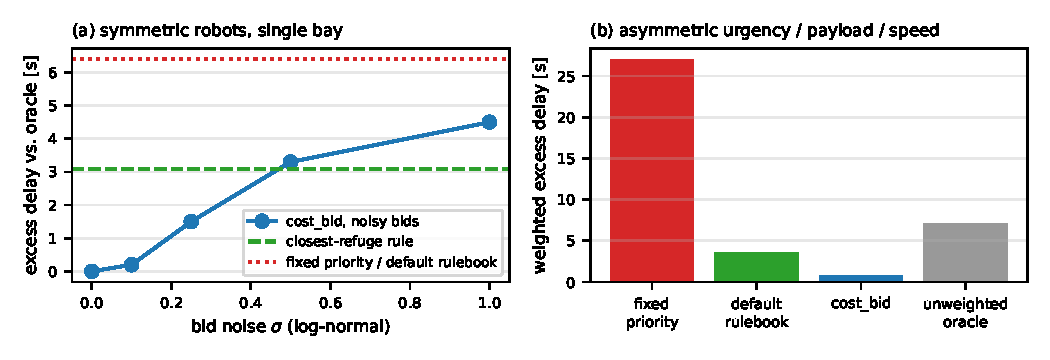
\includegraphics[width=0.95\columnwidth]{fig/results.pdf}
\caption{(a) Excess delay~\eqref{eq:excess} of \cb\ over the best forced yielder as bid noise grows, compared with two noise-free rulebooks. (b) Urgency-weighted excess delay with asymmetric robots. Bars and markers are means; error bars are 95\% confidence intervals. Values are computed from the released per-episode results.}
\label{fig:res}
\end{figure}

\subsection{Incentives and fairness}\label{sec:inc}
\emph{Misreporting under lower-bid-yields.} If B inflates its bid by $2\times$ or more, it never yields: its own delay falls from $9.1\pm1.4$ to $8.1\pm1.2$\,s while total delay rises by 4.9\,s (+20\%). Lower-bid-yields bidding is not incentive compatible. The naive transfer (Sec.~\ref{sec:pol}) is also gameable: A gained 7.5\,s by reporting $0.25\times$ its cost, and B 0.7\,s at $0.75\times$.

\emph{Clarke-pivot payments.} We scaled one or both robots' reports by $k\in\{0.25,\dots,4\}$ (10 values) over 3 bay positions, B urgency 1 and 3, and 60 draws. Each of the 6 configurations has 28 report profiles (A, B, or both deviating at each $k$, with the truthful profile run once), giving 10\,080 episodes, all successful. No unilateral misreport by A or B lowered the deviator's cost, its weighted delay plus payment, under the predicted costs; under the realized simulator delays the largest gain was 0.02\,s. The VCG theorem guarantees this result for any report scaling under the shared cost model, so these episodes confirm the implementation rather than add evidence for truthfulness. The tested deviations are also narrow. A robot could omit known bays from its BID, which changes the set of feasible outcomes over which $r_i(o)$ is defined, and Sec.~\ref{sec:maps} shows that the bays a robot lists change decisions. A lower-ID robot could also exploit the commit tie-break by announcing a decision that favors it. We assume robots follow the protocol apart from their cost reports and test neither manipulation. The mechanism is not budget balanced, consistent with~\cite{green1977characterization,myerson1983efficient}: the bank collects 9.3\,s (B urgency 1) and 10.5\,s (urgency 3) of credit per encounter, which a fleet would have to recycle as a virtual currency. Joint shading is profitable: if both robots report $0.5\times$, their combined utility improves by 4.9\,s. Payments are charged in credit, so a robot that expects a large payment may prefer not to participate; we do not analyze individual rationality.

\emph{Fairness.} Fixed priority makes B yield in every episode. Over 50 sequences of 20 repeated encounters, we measure each robot's delay for both yield decisions with forced-yielder runs and apply each selection rule offline to these measured costs; no payments are made. Cost-optimal choice already reaches a Jain index of 0.93 on cumulative delays; fixed priority costs 27\% more delay for 0.75, strict alternation 22\% for 0.99, and credit-weighted choice, which minimizes total delay plus $\lambda$ times the difference in cumulative delays, reaches 0.997 at $\lambda=0.25$ for 8\% extra delay. This is a simple instance of the credit schemes of~\cite{censi2019karma,elokda2024karma}. Fairness credit is distinct from Clarke payment credit; if Clarke credit were carried across encounters, a robot could bank it, and our single-encounter truthfulness analysis would no longer apply.

\subsection{Communication impairment}\label{sec:comms}
With 6\,m detection, loss up to 90\%, and latency up to 2\,s (3\,600 episodes), and with detection ranges of 1.5--6\,m at 0.26 or 0.5\,m/s under the same loss and latency limits (4\,320 episodes), every policy succeeded in at least 99.3\% of its episodes with no collisions. Under extreme conditions (loss 90--99\%, latency 2--8\,s, 0.5\,m/s, 1\,440 episodes), a pre-release version of the protocol collided in 6 episodes, each after both robots yielded on inconsistent decisions; this failure motivated protocol changes. With all three safeguards on, which is the default, the final code has no collisions in these 1\,440 episodes, and each of the four policies succeeds in 98.9--99.2\% of its episodes. We did not run the extreme grid at the Waffle's 0.26\,m/s in 2D; the milder grid includes both speeds, and the Gazebo extreme-comms runs use 0.26\,m/s (Sec.~\ref{sec:gz}).

Table~\ref{tab:abl} ablates the three safeguards on the same extreme grid (360 episodes per arm). No arm collided, including the one with all safeguards off (95\% upper bound 1.1\% per arm), so on the final code we cannot attribute collision avoidance to any single safeguard; the remaining protection comes from the yield and pass logic itself. With STATE sent at 5\,Hz and freshness counted from receipt, a robot holds no fresh STATE of its peer with probability $0.9^5$ to $0.99^5$, i.e.\ 59--95\% of the time, so the state-based checks act intermittently and on STATE content 2--8\,s old, and the lidar and the timers of Sec.~\ref{sec:proto} carry the rest. The lidar bay check never triggered, and its arms were identical episode for episode to those without it. With commit, fixed priority succeeded in 99.2\% of episodes against 98.1--98.6\% without it, whereas \cb's success rose slightly as safeguards were removed, from 98.9\% to 99.7\%; commit added 3--4\,s of mean delay for both policies. These success differences are 1--4 deadlocks in 360 episodes and lie within sampling noise, so commit did not measurably help either policy. In 14--24\% of episodes both robots started a yield before one gave way. The protocol does not guarantee that such mutual yields terminate, and we have no bound on how long such mutual yields last; the deadlocks in Table~\ref{tab:abl} are episodes that did not resolve within the 180\,s limit.

\begin{table}[t]\centering
\caption{Protocol ablation under 90--99\% loss and 2--8\,s latency (360 episodes per row; the bay check had no effect and is omitted). No row had a collision. The default protocol is the first row of each policy.}
\label{tab:abl}
{\footnotesize\setlength{\tabcolsep}{4pt}
\begin{tabular}{@{}lccrrr@{}}\toprule
Policy & Commit & State & Success [\%] & Deadl. & Delay [s]\\\midrule
Fixed priority & \checkmark & \checkmark & 99.2 & 3 & $89.8\pm3.9$\\
 & \checkmark & -- & 99.2 & 3 & $90.0\pm4.0$\\
 & -- & \checkmark & 98.1 & 7 & $86.0\pm3.6$\\
 & -- & -- & 98.6 & 5 & $86.8\pm3.7$\\\midrule
\cb & \checkmark & \checkmark & 98.9 & 4 & $79.6\pm3.9$\\
 & \checkmark & -- & 99.2 & 3 & $79.9\pm3.9$\\
 & -- & \checkmark & 99.4 & 2 & $76.4\pm3.7$\\
 & -- & -- & 99.7 & 1 & $76.8\pm3.7$\\\bottomrule
\end{tabular}}\\[2pt]
{\footnotesize State: state guard. Deadl.: deadlocks. Delay: mean total delay over successful episodes.}
\end{table}

\subsection{Three robots and junctions}\label{sec:three}
\emph{Convoy.} With a two-robot convoy against one oncoming robot (72 runs per policy and B type, pooled over 0\% and 50\% loss: 12 bay and start-delay combinations, each with 3 seeds that vary jitter and loss; Table~\ref{tab:design}), a yielding leader could be blocked by its own follower; a ``make room'' rule, in which the follower backs into its own refuge, removed these deadlocks, and every policy then succeeded in 72/72 runs. With equal urgency, pairwise \cb\ ignores the follower and averaged 55.6\,s total delay; \gb\ reduced this to 34.4\,s, 0.7\,s above fixed priority and the side-level reference (both 33.7\,s); the paired interval of this difference is $\pm1.4$\,s, so we do not claim the two are equivalent. When the lone robot is urgent ($u=3$), the side-level reference has 85.7\,s urgency-weighted delay, fixed priority 90.3\,s, \gb\ 104.7\,s, and \cb\ 117.1\,s (95\% CIs $\pm3.1$, $\pm4.2$, $\pm6.7$, $\pm6.3$\,s). \gb\ still underestimates what a convoy yield costs: paired per-draw intervals place it $14.4\pm8.0$\,s worse than fixed priority and $19.0\pm6.9$\,s above the side-level reference, with \cb\ a further $12.4\pm5.8$\,s above \gb. % VERIFIED 2026-10-23: rerun convoy per-episode results (means match report/convoy_group.txt); paired diffs per (x0,x1,start_delay,seed,loss) draw


\emph{T-junction.} With one robot turning into the branch, one passing, and one leaving the branch (48 runs per policy and loss level), naive waiting in the lane deadlocked fixed priority in 19 of 48 runs at 0\% loss. Letting the turning robot wait in a free bay before the junction gave 48/48 for fixed priority, the rulebook, and \cb\ at 0\% and 50\% loss, with mean delay over successes of 60.5, 53.1, and 48.9\,s (95\% CIs $\pm4.7$, $\pm5.0$, $\pm4.0$\,s; \cb\ below the rulebook by $4.3\pm2.8$\,s paired) at 0\% loss. % VERIFIED 2026-10-23: rerun tjunction_goal per-episode results, means match report/tjunction_goal.txt
The reactive baseline succeeded in 28/48. All failures in this study were deadlocks.

\subsection{Inconsistent and wrong maps}\label{sec:maps}
When robots know different bays (two-bay corridor, 840 episodes, 10 seeds per cell), map disagreement caused no collision or deadlock: commit detects the mismatch and both adopt the decision of A, the lower-ID robot. It costs time only when A has the poorer map, and not in every such condition: if A knows only bay 2 there is no cost. If A knows only bay 1, the excess over the full map is +9.1\,s for \cb\ and +29.6\,s for fixed priority and the default rulebook at 0\% loss (+9.3 and +29.3\,s at 50\%); if A knows no bay, all three lose 30.9--31.1\,s. Listing known bays in each BID removed the cost in every condition in which at least one robot knew a bay; when neither did, there was nothing to share. When the useful bay was physically blocked, every negotiating policy initially deadlocked (10/10), because the yielder's bay check mistook the obstacle for a robot. Distinguishing obstructions from robots via STATE messages and falling back to the next refuge restored 10/10 success with no collisions, at about +46\,s because the obstruction is discovered only on arrival. These samples are small.

\subsection{Exploring robots}\label{sec:explore}
In explore mode a robot starts knowing only the corridor and its end rooms and adds a bay to its map once the bay is within lidar range (3.5\,m). This is geometric discovery on a known layout, not SLAM. With share-on-detect, a robot sends its known bays only after its own lidar has detected the peer; STATE and BID messages flow as before. In the two-bay corridor (1\,440 episodes, 30 seeds per cell) every episode succeeded without collision. At the default 6\,m negotiation range, not sharing cost $+29.2$\,s for fixed priority and the rulebook and $+8.8$\,s for \cb\ against the full map, because each robot had seen only its nearest bay when they decided; sharing the map in every BID removed the cost. Share-on-detect equalled not sharing at 6\,m: the robots decide before either lidar can see the other, so the map never arrived in time (0/30). When negotiation started only at 3.5\,m, share-on-detect matched the full map in 2D. In Gazebo it did not: detection from lidar clusters first occurred 2.3--2.6\,m apart on average, after the decision, so the map again arrived late (0/6), and fixed priority's mean total delay was 7.0\,s above the Gazebo full-map run of the same seed (6.8\,s above the paired 2D run). Sharing on detection therefore helps only if detection reliably precedes the decision.

We therefore added an opt-in hold mode (\texttt{hold\_for\_map}, off by default). A share-on-detect robot postpones its decision, still driving its lane and refreshing its BID snapshot, until its own lidar has detected the peer and it has the peer's map (a MAP message, or a BID carrying the map). After a 15\,s timeout it decides as before. In 2D (360 extra episodes at 0 and 50\% loss) every hold episode succeeded, with no collision and no timeout. At 6\,m, holding removed share-on-detect's excess delay ($+29.2$\,s for fixed priority, $+8.8$\,s for \cb), ending 0.4--0.5\,s below the full map, at the cost of 4.9--5.5\,s from conflict to decision instead of 0.1--0.3\,s. At 3.5\,m it changed little ($+0.1$\,s against $+1.7$\,s for fixed priority at 50\% loss). In Gazebo (24 hold runs, seeds 0--5, 0\% loss, run with 12 share-on-detect reruns as a batch outside the 460 runs of Sec.~\ref{sec:gz}) every run succeeded without collision or timeout, and the yielder used the nearer bay in all of them, including the seed where share-on-detect had sent fixed priority's yielder to its end room. But the decision came 4.7\,s (3.5\,m) and 9.5\,s (6\,m) after the conflict began, because detection, the first lidar cluster within 0.5\,m of the peer's broadcast position, came only 1.1--1.2\,m apart in these runs, and each run took on average 4.7--4.9\,s (3.4--6.1\,s per run) longer than the paired 2D run. Detection uses the same test in the share-on-detect runs, where it came farther apart; we have not traced why holding delays it. % VERIFIED 2026-10-23: gz_detect_dist in report/gazebo_hold_runs.csv is 1.10--1.18 m on all 24 hold runs; it is the robot distance at the first peer_detected event (agent.py sense(): fresh STATE within lidar range and a cluster within 2r of the STATE position); share-on-detect reruns in the same file: 1.23--3.36 m
Against the Gazebo full-map run of the same seed, total delay was $+10.0$--$10.1$\,s for each policy; the values nearly coincide because with the hold both policies sent B into bay 2 in every run. This is more than share-on-detect without holding ($+7.0$\,s for fixed priority, $+0.3$\,s for \cb). At detection, A had already sensed both bays itself in all 6 seeds and B in 5 of 6, so in Gazebo the hold works by waiting, not through the exchanged map. Holding thus fixes the wrong-refuge failure but not its cost; sharing the map in every BID remains the cheaper fix in both simulators.

\subsection{Learned negotiator}\label{sec:learned}
The table was trained in the two-bay corridor with randomized bay positions, start delays, urgency, and payload. On 150 held-out encounters in that layout, it reached rulebook-level weighted excess delay (+2.6\,s, against +2.5\,s for the rulebook, +9.2\,s for fixed priority and 0.0\,s for \cb). On 150 encounters in the single-bay corridor with a randomly placed bay, a layout absent from training, it was no better than fixed priority (+13.1\,s against +12.3\,s), with 15\% of observations unseen, so it does not generalize across layouts.

\subsection{Gazebo validation}\label{sec:gz}
All Gazebo runs use the final agent code. In terms of the rows of Table~\ref{tab:gz}, 122 cases ran on the commit before the last two: 40 of the 70 single-bay negotiating runs (fixed priority, both rulebooks, \cb), the 10 reactive runs, 18 of the 36 convoy runs (fixed priority, rulebook, \cb\ with equal urgency), all 36 T-junction runs, and all 18 50\%-loss runs. The other 338 cases ran on the last commit; the last two commits add only explore mode and Gazebo support (blocked-bay obstacles, per-run policy files). A Gazebo run takes about 5\,min, so instead of the full 2D grids we ran every study's scenario on a reduced grid of 6--10 seeds per condition, each paired with a 2D run on the same seed (Table~\ref{tab:gz}). Extreme comms used the Waffle's 0.26\,m/s rather than 0.5\,m/s, and the protocol ablation was reduced to all safeguards on and all off. Seeds fix the start delays, but Gazebo physics and ROS timing are not deterministic, so each case is a single sample.

Across the 450 runs other than the reactive baseline (negotiating policies and forced yielders) there were no failures and no collisions (95\% upper bound 0.85\%), including the blocked bay, where touching the obstacle counts as a collision. Excluding the 44 forced-yielder runs, whose first yielder is fixed by construction, 393 of the 406 negotiating runs (96.8\%) chose the same first yielder as 2D. Of the 13 differences, 5 are noisy-bid runs, whose noise draw is keyed to the decision time, which differs between the simulators, 6 are 90\%-loss runs, whose loss realizations differ, and one each is a T-junction and an explore run. Where the two simulators share the random draws, excess delay against each simulator's own best forced yielder transferred: for every policy in the single-bay, unequal-urgency and slow-robot cases it was within 1.0\,s of the 2D value (e.g.\ fixed priority 7.5 vs 7.6\,s, reservation 15.2 vs 15.2\,s, learned 5.1 vs 5.3\,s, \cb\ and Clarke 0 in both). In the other non-reactive groups, mean Gazebo delays were 0.2--1.2\,s lower than in 2D; the exceptions are the T-junction, the noisy-bid and 90\%-loss cases, where the differing draws dominate, and share-on-detect in explore mode (Sec.~\ref{sec:explore}).

The T-junction did not transfer. Its delay difference summed over the 36 runs is $-605.3$\,s (mean $-16.8$\,s); $-260.0$\,s comes from the 18 exit runs and $-345.4$\,s from the 18 turn-in runs. When the branch robot leaves the branch, \cb\ finished 22\,s earlier on average in Gazebo (11--75\,s), and a second robot also yielded in Gazebo in 4 of 4 fixed-priority and 3 of 4 rulebook runs whose paired 2D run had a single yielder. Both differences trace to one timing race: whether the branch robot leaves the stem before or after A clears the bay. Under \cb\ A is the first yielder and waits parked off the lane; under fixed priority and the rulebook B yields and A holds in the lane. In 2D the two events coincide: A and the branch robot meet head-on, negotiate a second time, and A yields again (about 20\,s; in one run both enter proceed at once and wait out the 60\,s proceed timeout---196.8\,s summed delay). In Gazebo the branch robot leaves about 20\,s earlier relative to A's parked window and passes the still-parked A without a second conflict; under fixed priority and the rulebook it leaves early enough to meet A holding in the lane, so it must yield into the stem a second time, whereas in 2D its first yield stays pending until A has passed. The cause is the order in which each simulator's communication and perception timing releases the branch robot, not a protocol difference. This account covers the exit runs (\cb\ $-264.7$\,s, fixed priority $+18.6$\,s, rulebook $-14.0$\,s). The larger turn-in share is unexplained: Gazebo delays were 9.5--11.7\,s lower per run where A yielded and 21.2--28.9\,s lower where B yielded (makespans 0.4--1.0 and 4.0--6.4\,s shorter), and we have not traced whether the same release offset causes this. We do not claim that T-junction delays transfer. Gazebo runs made before the final code exposed two sim-to-real gaps at the T-junction: a goal on the room wall was ``reached'' in 2D, which has no wall perception, and the branch walls occlude the lidar of a robot inside it. Both fixes are in the final code; they were found and checked on the same cases, so the T-junction rows are not an independent validation. % VERIFIED 2026-10-23: traced final-code runs — 2D s3 events show both A and S entering proceed at t~37.4, proceed_timeout at 97.35; gz_tj runs show S exiting bay1 ~20 s earlier relative to A's parked window; variant sums from report/gazebo_main_runs.csv gz_wdelay-d2_wdelay: tj -260.0 (cb -264.66, fp +18.64, rd -13.97), tjgoal -345.35; tjgoal makespan d2-gz 0.448--6.4 s; proceed_timeout -> fallback_reactive (agent.py tick_proceed)


\begin{table}[t]\centering
\caption{Gazebo runs on the final code, each paired with a 2D run on the same seed.}
\label{tab:gz}
{\footnotesize\setlength{\tabcolsep}{4pt}
\begin{tabular}{@{}lrrrrr@{}}\toprule
Scenario & Runs & Succ. & Coll. & Same & $\Delta D$ [s]\\\midrule
Single bay, negotiating & 70 & 70 & 0 & 70 & $-0.4$\\
Single bay, reactive & 10 & 9 & 1 & 5 & $-1.5$\\
Single bay, forced yielder & 44 & 44 & 0 & 44 & $-0.5$\\
Unequal urgency or speed & 36 & 36 & 0 & 36 & $-0.6$\\
Two bays & 30 & 30 & 0 & 30 & $-0.2$\\
Noisy bids ($\sigma=0.5,1$) & 12 & 12 & 0 & 7 & $+2.2$\\
Clarke misreports & 18 & 18 & 0 & 18 & $-0.3$\\
50\% loss & 18 & 18 & 0 & 18 & $-0.8$\\
90\% loss, 2\,s latency & 24 & 24 & 0 & 18 & $+4.8$\\
Convoy (2 v 1) & 36 & 36 & 0 & 36 & $-0.6$\\
T-junction & 36 & 36 & 0 & 35 & $-16.8$\\
Different known bays & 24 & 24 & 0 & 24 & $-0.3$\\
Blocked bay & 18 & 18 & 0 & 18 & $-1.2$\\
Explore & 84 & 84 & 0 & 83 & $+0.2$\\\bottomrule
\end{tabular}}\\[2pt]
{\footnotesize Succ.: success. Coll.: collisions. Same: same first yielder as 2D (fixed by construction for forced yielders). $\Delta D$: mean Gazebo minus 2D (urgency-weighted) total delay. The 50\% loss runs also have 0.5\,s latency.}
\end{table}

\section{Discussion and Limitations}
Three conclusions hold across our studies. First, communication is cheap insurance: in the corridor studies every negotiating policy avoided the deadlocks and back-off ``dances'' of the reactive baseline, though our data do not separate message value from a shared deterministic rule. Second, the right rule depends on what the robots know: cost bidding is best when robots differ and their bids match the simulator's cost model to within a scalar log-normal error of $\sigma\approx0.25$, but it needs payments to resist misreporting and side-level costs to approach the convoy reference, and even our group bid trails fixed priority by $14.4\pm8.0$\,s when the lone robot is urgent. Third, under extreme packet loss our protocol had no collisions, but the ablation shows that this cannot be credited to the commit step or the bay check alone.

The study has clear limits. All results are from simulation. The Gazebo runs cover a reduced grid with one non-deterministic run per case (6--10 seeds per condition), the T-junction turn-in delay gap is unexplained (the exit share is a release-timing race), and physical TurtleBot3 trials are future work. \cb\ and the Clarke mechanism use the simulator's own motion model, so their efficiency and truthfulness hold relative to that model only; structural model errors, misreported refuge sets, and abuse of the commit tie-break are untested, and the mechanism neither balances its budget nor resists collusion. The only non-communicating baseline is reactive; no ORCA/RVO/CBF controller was run, so the motivating deadlock is taken from the literature. The protocol has no formal safety or liveness guarantee. The best forced yielder is a reference for the yield decision, not a global optimum, and only the convoy has a three-robot reference. The T-junction is approximated as a deep bay, explore mode discovers bays geometrically rather than by SLAM, and the map studies use 10 seeds per cell. The learned baseline is tabular and centrally trained, and LLM negotiators~\cite{marlin2024,gamechat2025} are untested.

\section{Conclusion}
We presented a benchmark for head-on corridor encounters with pull-in bays and compared negotiation policies under identical physics and communication models. When its bids use the simulator's own cost model, cost bidding matches the best forced yielder and handles asymmetric robots, and it loses that advantage over a closest-refuge rule at a log-normal bid error of $\sigma=0.5$. Under the same model, Clarke-pivot payments remove the gain from scaled unilateral misreports at the price of a budget surplus; a small fairness credit makes repeated encounters fair for 8\% extra delay; and, in our layout, first-come reservation and fixed priority leave 6--19\,s of excess delay per encounter. The simulator, ROS~2 nodes, scenarios, study scripts, and results are released at \url{[ANONYMIZED-URL]} to support comparison with learned and language-model negotiators.

\bibliographystyle{IEEEtran}
\enlargethispage{6\baselineskip}
\bibliography{refs}
\end{document}
